\documentclass[a4paper, dvipsnames, table]{article} 
\usepackage{Stiletemplate}
\usepackage[utf8]{inputenc}
\usepackage[T1]{fontenc}
\usepackage[italian]{babel}
\usepackage{graphicx}
\usepackage{fancyhdr}

\pagestyle{fancy}

\begin{document}
\copertina

\newpage
\tableofcontents

\newpage
Il progetto \emph{Burgheria Padovana} vuole implementare un sito Internet che offra la possibilità di fornire informazioni riguardo il suo punto vendita.\\
Il locale è aperto già da diversi anni e ha finalmente deciso di rinnovarsi creando un proprio sito internet.\\
Il sito dovrà contenere informazioni riguardanti i panini che offre, suddivisi nelle varie categorie: Pollo, Manzo e Speciali. 
Inoltre conterrà gli eventi a cui sarà possibile partecipare, la storia del locale, gli orari di apertura e come contattare il locale.\\
Il sito permette ad un utente privilegiato (admin) di inserire o eliminare gli eventi e di controllare ed eliminare i commenti degli altri utenti. Gli utenti normali (user) saranno visitatori 
con privilegi minimi per poter inserire od eliminare i propri commenti oltre a poter visitare il sito normalmente.\\
Gli \emph{user} dovranno effettuare la registrazione o il login prima di poter usufruire dei privilegi.\\
Inoltre deve essere garantita l'accessibilità in modo che chiunque possa navigare nel sito senza problemi e tranquillamente.\\
Terminato con l'accessibilità, si pone l'attenzione sull'usabilità: rispettando la separazione tra struttura, presentazione e comportamento e rispettando gli standard \emph{W3C} per quanto riguarda \emph{HTML} e \emph{CSS}.\\
Il sito dovrà garantire una navigazione fluida agli utenti evitando disorientamento e, nel caso accadesse, fornirgli supporto per tornare al sito.\\

\newpage
\section{Analisi}
Il locale Burgheria Padovana offre un prodotto internazionale, comodo, veloce e buono.\\
Pertanto il sito è pensato per rivolgersi ad una categoria di utenti eterogenei, ad esempio: da consumatori abituali a chi vuole provare qualcosa di nuovo, da chi ha bisogno di mangiare qualcosa al volo a chi vuole gustarsi un buon pasto con calma.\\
Queste categorie di utenti, con privilegi minimi, verrà denominata come \emph{utente generico}.
Mentre l'utente con privilegi verrà denominato come \emph{amministratore}.\\ 
Entrambe le tipologie potranno accedere ai loro privilegi autenticandosi tramite form di login.\\
Essendo un utenza finale generica, sarà necessario utilizzare un linguaggio informale, semplice e comprensibile.
Allo stesso modo si andrà a creare un sito di struttura e layout semplici e simili ai modelli a cui l'\emph{utente generico} è abituato.
Si cercherà, quindi, di non rompere le convenzioni esterne e offrendo, indipendentemente dal browser o dal dispositivo utilizzato, una navigazione veloce e intuitiva.\\
Sia l'\emph{utente generico} sia l'\emph{amministratore} possono visitare tutte la pagine del sito e una volta eseguito il \emph{login} o la \emph{registrazione} accedono ai relativi privilegi.
Le differenze tra le due tipologie di utenti sono le seguenti:
\begin{itemize}
	\item La pagina \emph{gestioneEventi} è visibile solo all'\emph{amministratore} dalla quale può aggiungere od eliminare nuovi eventi.
	\item La pagina \emph{gestionePanini} è visibile solo all'\emph{amministratore} dalla quale può aggiungere od eliminare nuovi panini.
	\item Nella pagina \emph{gestioneCommenti} l'\emph{utente generico} vede e gestisce i commenti lasciati solo da lui, mentre l'\emph{amministratore} vede e gestisce i commenti di tutti gli utenti.
\end{itemize}

\newpage
\section{Progettazione}
Il progetto \emph{Burgheria Padovana} si prefigge di rispettare le specifiche tecniche richieste:
\begin{itemize}
	\item \textbf{Rispettare gli standard:}\\ 
	È stato scelto di utilizzare \emph{HTML5} per il contenuto e \emph{CSS3} per la presentazione.
	\item \textbf{Separazione tra contenuto, presentazione e comportamento:}\\ 
	Per il contenuto è stato utilizzato \emph{HTML}, per la presentazione è stato utilizzato \emph{CSS} e per il comportamento è stato utilizzato \emph{PHP} e \emph{JavaScript}.
	\item \textbf{Accessibilità:}\\ 
	Il sito è stato progettato per permettere a tutte le categorie di utenti di accedere al sito.
	Per fare ciò si è scelto uno sviluppo del sito rispettando fin dal principio norme e pratiche per facilitare l'accessibilità.
	In questo modo si riduce il lavoro di controllo e validazione per quanto riguarda l'accessibilità evitando di dover riscrivere parti di codici che potrebbero causare problemi di accessibilità.
	\item \textbf{Usabilità:}\\
	Il sito è stato progettato per permettere una navigazione fluida, semplice e tradizionale per evitare all'utente disorientamento e sovraccarico cognitivo.
	\item \textbf{PHP e DB:}\\
	Sono state utilizzate pagine in \emph{PHP} per poter interagire con il \emph{DB} ottenendo, scrivendo o eliminando dati. Sarà utilizzato un \emph{DB} in forma normale dove salvare eventuali dati inseriti dagli utenti.
	\item \textbf{Form:}\\
	Sono stati implementati controlli dell'input da parte dell'utente sia lato client (\emph{PHP}) sia lato server (\emph{JavaScript}).
	\item \textbf{Dispositivi:}\\
	Il sito è stato progettato per essere utilizzato da diversi dispositivi e a diverse dimensioni senza problemi. Per fare ciò si è utilizzato la pratica di sviluppo "\emph{Mobile First}" con la quale il progetto viene ideato pensando prima a dispositivi mobile.
\end{itemize}
Per rendere il sito accessibile e usabile sono state applicate le seguenti scelte: 
	\begin{itemize}
		\item Utilizzo dell'attributo \emph{alt} nelle immagini, per persone con disabilità visive.
		 Tale attributo permette di inserire delle descrizioni delle immagini che verranno poi lette dal screen reader. 
		 La descrizione deve essere riportata solo se l'immagine è di contenuto e riporta informazioni importanti altrimenti, se l'immagine è solo di presentazione, la descrizione viene lasciata vuota.
		 Inoltre se si decide di implementare la descrizione, quest'ultima deve essere chiara ed esaustiva per non confondere l'utente.
		\item Utilizzo di \emph{aiuti nascosti}, per persone che utilizzano screen reader o navigazione tramite tastiera. 
		Gli \emph{aiuti nascosti} sono link invisibili all'utente ma visibile agli screen reader.
		 Sono utilizzati in diversi punti della pagina e permettono di saltare contenuti non interessanti e dirigersi direttamente a ciò che si cerca.
		\item Attenzione ai contrasti dei colori, per evitare problemi o disorientamento a utenti daltonici. 
		\item Per aiutare l'utente a capire dove si trova viene sottolineato nel menu la pagina in cui si trova l'utente; inoltre nella pagina \emph{Menu} viene sottolineata la categoria che l'utente sta visualizzando.
		Per i link presenti nel contenuto viene utilizzata la convezione standard: sono colorati di blu se non sono stati visitati altrimenti sono viola.
		I link dei bottoni del menu non seguono questa convezione poiché facilmente riconoscibili.
		\item Nelle form, quando l'utente sbaglia, vengono riportati avvisi di errore spiegando cosa è stato sbagliato facilitando la comprensione dell'utente ed evitando disorientamento.
		\item Non è stato necessario l'implementazione di \emph{tabindex}, in quanto l'ordine seguito è logico e rispetta l'ordine dei contenuti della pagina. % da decidere se usare o meno
		\item Nelle pagine \emph{Panino} e \emph{gestioneCommenti} è stato utilizzato il bottone \emph{torna su}; Questo bottone posto in fondo alla pagina, sotto ai commenti, è un link che permette all'utente di ritornare a inizio pagina evitando scroll inutile e velocizzando la navigazione. 
		\item Per la versione \emph{Mobile} è stata rispettata la "Comfort Zone" ossia il menu, le form, link o altre opzioni cliccabili sono state inserite in zone comode da raggiungere per l'utente. 
	\end{itemize}
\subsection{Design}
Come già dichiarato sono state seguite due strategie per la creazione del sito: \emph{Mobile First} e l'attenzione fin dall'inizio all'accessibilità.\\
È stato scelto un \emph{layout a quattro pannelli} per la maggior parte delle pagine, che si adatta facilmente alla strategia di \emph{Mobile First}.\\
L'unica eccezione è la pagina \emph{Menu} che usa un \emph{layout a cinque pannelli} per poter inserire il menu categoria lateralmente.\\
I pannelli presenti nel layout sono, in ordine di presentazione:
\begin{enumerate}
	\item \textbf{header:} contiene il logo e il nome del Locale e contiene il menu; 
	\item \textbf{breadcrumb:} contiene il percorso della pagina corrente, serve ad orientare l'utente all'interno del sito;
	\item \textbf{contenutoGenerale:} contiene le informazioni principali della pagina visitata;
	\item \textbf{footer:} contiene le informazioni di contatto e la partita IVA del locale;
	\item \textbf{leftSideBar:} nella versione \emph{Desktop} è utilizzata solo dalla pagina \emph{Menu}.
	 Si trova, come suggerisce il nome, a sinistra del \emph{contenutoGenerale} e contiene la selezione della categoria dei panini. 
	Nella versione \emph{Mobile} si trova invece tra il pannello \emph{breadcrumb} e il pannello \emph{contenutoGenerale}.
\end{enumerate}
Una parte fondamentale del progetto è il database, in quanto è usato per contenere le informazioni che veranno poi usate dal sito.\\
È stato pensato di creare un database con la funzione di contenere tutti i dati relativi ai prodotti in vendita compresi i voti e i commenti, agli eventi a cui è possibile partecipare e i dati degli utenti registrati.\\
Come si può vedere dalla \emph{Figura \ref{Fig:schemadb}}, le tabelle sono sei:
\begin{itemize}
		\item \textbf{Eventi:} contiene il titolo, la data, il luogo e la descrizione degli eventi a cui sarà possibile partecipare
		\item \textbf{Categoria:} contiene il nome delle categorie
		\item \textbf{Prodotti:} contiene il nome, l'immagine, gli ingredienti e la descrizione dei prodotti venduti
		\item \textbf{Utenti:} contiene l'username e la password degli utenti iscritti. Inoltre si verifica se l'utente è un admin.
        \item \textbf{Voti:} contiene i voti degli utenti
        \item \textbf{Commenti:} contiene i commenti degli utenti
\end{itemize}
\begin{figure}[!h]
	\centering	% L'immagine aggiornata è presente nel branch Main
	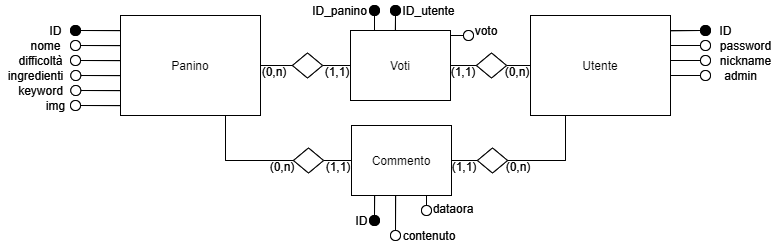
\includegraphics[width=0.7\linewidth]{../database/DiagrammaER.png}\\
    \caption{Schema concettuale database}
	\label{Fig:schemadb}
\end{figure}
Il database viene interrogato da PHP quando bisogna utilizzare o richiamare le informazioni.
Le pagine: \emph{Eventi}, \emph{I nostri Burger}, \emph{Panino} sono riempite dinamicamente tramite chiamata \emph{PHP}.\\
Come spiegato nella sezione \emph{Analisi}, esistono due tipi di utenti: \emph{utente generico} e \emph{amministratore}. Nel database viene utilizzato un booleano per differenziare le due tipologie.\\ 

\newpage
\section{Presentazione}
Si è deciso di utilizzare una dimensione massima di 1024px in modo che la pagina non risulti eccessivamente grande evitando così l'eventuale sforzo fisico dell'utente nel visionare l'intera pagina.\\
Caratteristiche della versione desktop:
\begin{itemize}
	\item Il logo del locale è presente;
	\item Il menu si presenta orizzontale tra il nome del locale e il breadcrumb.
\end{itemize}
Per facilitarne l'utilizzo e rendere accessibile il sito da \emph{mobile} è stato deciso di apportare alcune modifiche rispetto alla versione \emph{Dekstop}.\\
È stato necessario utilizzare due punti di rottura per le dimensioni dello schermo:
\begin{itemize}
	\item Un max-width di 730px
	\item Un max-width di 694px
\end{itemize}
In base al punto di rottura avvengono determinate modifiche allo stile delle pagine:
\begin{itemize}
	\item \textbf{730px}
	\begin{itemize}
		\item L'unica modifica, a questo punto di rottura, riguarda la pagina \emph{Menu} dove la sezione verticale a sinistra del \emph{contenutoGenerale}, usata per la selezione della categoria, viene spostata al di sopra del \emph{contenutoGenerale};
Viene trasformata in una sezione orizzontale tenendo la linea di separazione tra questa sezione e il \emph{contenutoGenerale}, presente anche nella versione \emph{Desktop}. 
In questo modo viene facilitata la visione e l'utilizzo da \emph{mobile}.
	\end{itemize}
	\item \textbf{694px}
	A questo punto di rottura avvengono diverse modifiche:
	\begin{itemize}
		\item Il logo del locale viene rimosso;
		\item Il menu orizzontale viene trasformato in un menu a tendina(tramite \emph{CSS}), con apertura verticale, adattandosi all'utilizzo da \emph{mobile};
		\item La pagina \emph{Panino} viene riadattata per un utilizzo migliore da \emph{mobile};
		\item La pagina \emph{Contatti} viene riadattata per un utilizzo migliore da \emph{mobile}, verticalizzando il contenuto;
		\item La pagina \emph{gestioneEventi} viene riadattata per un utilizzo migliore da \emph{mobile}, verticalizzando le form.
	\end{itemize}
\end{itemize}
Per la stampa abbiamo eliminato tutte le funzioni interattive lasciando solo il contenuto di interesse.
Questo perché nessuna delle form richiedeva troppi dati(non serve stampare la form per preparare tutti i dati da inserire in seguito).\\
Sono stati eliminati background, colori, sottolineature non necessarie, immagini non importanti, eventuali aiuti nascosti, le icone del menu a tendina, il breadcrumb ed è stato utilizzato uno stile \emph{serif} per la scrittura.\\
È stata presa la decisione di lasciare alcuni link sottolineati per far sapere all'utente la presenza di eventuali pagine che non ha visitato ma che potrebbero interessargli. %Da rivedere parte link
Sono state modificate le dimensioni di alcune scritte e lo spazio in alcune pagine è stato riadattato.\\
È stata fatta la scelta di mantenere le immagini dei panini nella pagina \emph{Menu}; 
questo perché la pagina viene usata come vetrina per mostrare i prodotti che vendiamo.
Inoltre al cliente potrebbe interessare stampare la vetrina dei prodotti per poter decidere in seguito.\\
La foto dei panini è stata tolta dalla pagina \emph{Panino} poiché si è ritenuto che se un utente stampa questa pagina ha già deciso che panino prendere e può essere interessato a stampare per diversi motivi, ad esempio:
\begin{itemize}
	\item Potrebbe stampare la pagina per potersi ricordare il nome del panino;
	\item Potrebbe essere interessato alla lista ingredienti in caso dovesse ricordarsi di richiedere l'eliminazione di un ingrediente per il suo ordine;
	\item Potrebbe voler stampare un commento ritenuto offensivo e avere una prova cartacea;
\end{itemize}

\newpage
\section{Implementazione}
È stato deciso di utilizzare il linguaggio \emph{HTML5} per diversi motivi:
\begin{itemize} %magari trovare altri motivi
	\item \emph{HTML5} è oramai supportato dalla maggior parte dei Browser Web;
	\item Dopo un sondaggio proposto alla clientela, è stato riscontrato che il 70\% dei nostri clienti sceglie di mangiare da noi quando si trova fuori casa. 
	Quindi la maggior parte dei nostri clienti utilizzerebbe il telefono per visitare il sito;
	\item La maggior parte degli accessi al web avviene tramite mobile;
\end{itemize}
Gli ultimi due punti si concentrano sull'utilizzo di un dispositivo \emph{Mobile} come strumento per visitare il futuro sito; questo è importante perché la maggior parte dei dispositivi \emph{Mobile} utilizza Browser aggiornati e quindi che supportano \emph{HTML5}.\\
Si tiene a precisare che in ogni caso viene rispettata la sintassi \emph{XHTML} e in caso il browser non supporti \emph{HTML5} il sito degraderà in modo elegante.\\
Inoltre si è scelto di utilizzare \emph{HTML5} per la sua fluidezza e funzionalità aggiuntive. %verificare
Esiste una pagina \emph{HTML5} per ogni pagina del sito.\\ %decidere se mettere o meno
Come linguaggio di stile è stato usato \emph{CSS3}.\\
È stata mantenuta la separazione tra struttura e presentazione utilizzando i seguenti accorgimenti: 
\begin{itemize}
    \item Non sono stati usati tag di stile nelle pagine \emph{HTML};
    \item Per la presentazione sono stati utilizzati file esterni senza utilizzare codice a cascata inline o embedded.
\end{itemize}
Ogni singola regola è stata valutata prima di utilizzarla, in base alla compatibilità dei browser.
In alcune parti del sito sono state utilizzate le flex invece delle grid poichè supportato maggiormente.\\
Nella maggior parte dei casi viene utilizzata come unità misura gli em o la percentuale.\\
Questo migliora l'accessibilità e garantisce una corretta visualizzazione delle pagine su tutti i formati di schermi.\\
I fogli di stile utilizzati sono tre:
\begin{itemize}
	\item Un foglio style.css per le impostazioni di stile generale;
	\item Un foglio mobile.css per le impostazioni di stile che riguardano il mobile, separando i diversi punti di rottura; %magari impostare meglio frase
	\item Un foglio print.css per le impostazioni che riguardano la stampa.
\end{itemize}
\subsection{MySQL}
Per il mantenimento e salvataggio dei dati e delle informazioni, si è deciso di utilizzare \emph{MySQL}\\
Per le funzioni che necessitano l'uso di \emph{MySQL} viene implementato l'estensione \emph{mysqli}\\
Il database utilizzato è descritto nel capitolo 3: \emph{Progettazione -> Database}.
\\
Da notare che alcuni campi per l'inserimento hanno una grandezza maggiore di quella limite imposta all'utente. 
Questo per assicurarci che anche usando tag HTML, dato che in \emph{MySQL} i simboli "<" e ">", le lettere accentate e caratteri speciali vengono tradotti occupando più spazio, ci sia il rischio che l'input non venisse accettato dal DB portando ad un rifiuto dell'inserimento.
È stato deciso di elaborare tutte le pagine in \emph{PHP}. Questa operazione è necessaria in quanto ogni 
pagina viene riportato il tasto di login se l'utente non è loggato, altrimenti ne viene mostrato l'username.\\
Il linguaggio \emph{PHP} viene utilizzato per leggere, ricavare, scrivere ed eliminare informazioni dal database.\\
Il sito è strutturato in questo modo: 
\begin{itemize}
    \item File \emph{HTML} per ogni singola pagina contenente tutte le parti statiche;
    \item I relativi file in \emph{PHP}, per elaborare le parti dinamiche e ritornare la pagina completa;
    \item File \emph{PHP} per la gestione di diverse funzionalità: inserimento o eliminazione di eventi, login e logout, la possibilità di votare o commentare un panino;
    \item File \emph{PHP} per l'interazione con il \emph{DB}.
\end{itemize}
In questo modo si mantiene la separazione tra struttura e comportamento, in quanto la struttura viene descritta nei file HTML, mentre il comportamento è gestito dai file \emph{PHP} e \emph{JS} come vedremo in seguito.\\

Nei file \emph{PHP} vengono eseguiti controlli lato client sull'input delle form controllando che i dati inseriti siano corretti e cercando di ridurre al minimo possibili tentativi di \emph{SQL injection}.\\
I metodi utilizzati per il controllo dell'input sono: 
    \begin{itemize}
        \item \emph{trim()}: elimina gli spazi prima e dopo la stringa in input;
        \item \emph{htmlentities()}: converte tutti i possibili caratteri speciali in entità \emph{HTML};
        \item \emph{strip\_tags()}: elimina tutti i possibili tag \emph{HTML};
        \item Inoltre viene utilizzata la funzione \emph{mysqli real escape string};
        \item Nella query per il login viene utilizzato \emph{BINARY} per rendere la form case sensitive;
    \end{itemize}
\emph{JavaScript} è un linguaggio che si occupa del comportamento del sito.\\
Nel nostro caso \emph{JavaScript} viene usato per effettuare controlli sulle form e per alcune feature:
\begin{itemize}
    \item nella pagina \emph{Panino} viene usato per verificare che il commento da inserire rispetti alcune condizioni e in caso contrario l'utente viene avvisato;
    \item nella pagina \emph{Panino} viene usato per il bottone "carica altri commenti";
    \item nella pagina \emph{gestioneEventi} viene usato per controllare che i dati immessi nella form \emph{Aggiungi evento} siano corretti, in caso contrario l'utente viene avvisato;
    \item nella pagina \emph{gestioneEventi} viene usato per prendere dal DB le date relative all'evento che si seleziona nella form di eliminazione;
    \item nella pagina \emph{gestioneCommenti} viene usato per il bottone "carica altri commenti" e per l'eliminazione dei commenti.
\end{itemize}

%Magari aggiungere perchè si usa il bottone "carica altri commenti"

\newpage
\section{Validazione}
La validazione è uno passo fondamentale del progetto, poiché serve a verificare che siano rispettati gli standard \emph{W3C} per quanto riguarda \emph{HTML} e \emph{CSS}.\\
Infatti rispettarli assicura un codice pulito, corretto e che favorisca l'accessibilità e l'usabilità.\\
Inoltre assicura:
\begin{itemize}
	\item Un alto livello di compatibilità tra i diversi browser, rendendo minime o nulle le differenze di visualizzazione del sito, sempre considerando la possibile versione del browser utilizzato dall'utenza a cui ci si riferisce;
	\item Essendo valido non dovrebbe contenere errori e quindi la navigazione risulta più veloce e fluida;
	\item Un sito valido e senza errori non viene interpretato dal browser "a modo suo" ma rispetta "il volere" degli sviluppatori comportandosi come previsto da questi ultimi;
	\item Un sito valido e senza errori viene indicizzato in modo positivo dal browser;
	\item Un sito più accessibile e usabile.
\end{itemize}
Per validare il sito sono stati utilizzati i seguenti strumenti:
\begin{itemize}
	\item \textbf{W3C HTML Validator}\\
	Indirizzo sito web: \url{https://validator.w3.org/}\\
	È un servizio gratuito di \emph{W3C} che consente di validare le pagine \emph{HTML}.
	La validazione può avvenire in tre modi: attraverso il caricamento del file da validare, facendo copia e incolla del codice da validare o inserendo l'indirizzo della pagina se quest'ultima si trova online.\\
	Se il codice non è valido, viene segnalato il numero di errori, il loro tipo e a quale riga e colonna della pagina sono stati trovati.
	\item \textbf{W3C CSS Validator}\\
	Indirizzo sito web: \url{https://jigsaw.w3.org/css-validator/}\\
	È un servizio gratuito di \emph{W3C} che consente di validare il \emph{CSS}.\\
	Anche in questo caso i metodi di validazione sono tre come nel sito precedente.\\
	La segnalazione degli errori viene gestita nell'identico modo del sito precedente.\\
	 \item In entrambi i siti, se le pagine e il codice risultano validi, riportano del codice \emph{HTML} per poter utilizzare delle immagini, del \emph{W3C},che certificano la validazione del sito.
\end{itemize}

\newpage
\section{Fase di Test e Strumenti}
\subsection{XAMPP}
\emph{XAMPP} è una distribuzione di Apache che permette, tra le varie funzioni, l'utilizzo di \emph{MySQL} e \emph{PHP} di cui abbiamo usufruito.\\
Il loro utilizzo ci ha permesso di realizzare in locale la parte dinamica del sito e la parte di Database, testando le richieste \emph{PHP} e le interrogazioni \emph{MySQL}.
È un plugin del browser Google Chrome, che permette di testare la navigazione del sito attraverso l'attivazione di varie disabilità capendo se il sito risulta accessibile.
\begin{itemize}
	\item Permette di verificare che il sito sia usufruibile e di facile 	lettura per persone con dislessia.\\
	\item Può simulare la visualizzazione del sito da parte di persone daltoniche verificando che sia utilizzabile da queste ultime.\\
	\item Può simulare la visualizzazione del sito da parte di persone con la cataratta e verificare che sia accessibile per loro.
	\item Può simulare la visualizzazione del sito da parte di persone con perdita di visione periferica o perdita di visione centrale verificando che possano accedere ed utilizzare il sito.
	\item Può simulare uno screen reader, verificando che sia di facile lettura a quest'ultimo e non ci siano problemi di perdita di focus, che ogni parte del sito sia capibile solo attraverso l'utilizzo di uno screen reader e che questo permetta l'uso di ogni funzione del sito.
\end{itemize}
Il fine ultimo per l'utilizzo di questo plugin è di rendere il sito accessibile a più categorie di utenti possibili cercando di prendere in considerazione tutte le disabilità che rendono complicato l'utilizzo del browser.\\
È un strumento molto potente che consente un validazione ottimale delle pagine Web, capendo se sono accessibili.\\
Le sue funzioni sono:
\begin{itemize}
	\item Controlla che il codice \emph{HTML} rispetti gli standard.
	\item Controlla che il codice \emph{CSS} rispetti gli standard.
	\item Controlla che vengano rispettate le regole di accessibilità, verifica che siano rispettare le \emph{WCAG} e utilizza \emph{AIRA} test.
	\item Controlla che i link funzionino.
\end{itemize}

\newpage
	\textbf{Albiero Davide}
	\begin{itemize}
		\item Progettazione iniziale
		\item Sviluppo codice HTML
		\item Sviluppo codice CSS
		\item Sviluppo DB
		\item Sviluppo codice PHP
		\item Sviluppo codice JS
		\item Validazione delle pagine
		\item Test di accessibilità
		\item Test di usabilità
	\end{itemize}	
	\textbf{Fincato Alessandro}
	\begin{itemize}
		\item Progettazione iniziale
		\item Sviluppo codice HTML
		\item Sviluppo codice CSS
		\item Sviluppo DB
		\item Validazione delle pagine
		\item Test di accessibilità
		\item Test di usabilità
	\end{itemize}	
	\textbf{Panighel Cristiano}
	\begin{itemize}
		\item Progettazione iniziale
		\item Sviluppo codice HTML
		\item Sviluppo codice CSS
		\item Validazione delle pagine
		\item Test di accessibilità
		\item Test di usabilità
	\end{itemize}	
	\textbf{Tossuto Matteo}
	\begin{itemize}
		\item Progettazione iniziale
		\item Sviluppo codice HTML
		\item Sviluppo codice CSS
		\item Sviluppo DB
		\item Sviluppo codice PHP
		\item Validazione delle pagine
		\item Test di accessibilità
		\item Test di usabilità
		\item Stesura Relazione
	\end{itemize}

Queste sono le principali attività svolte dal singolo membro del gruppo.\\
Tutti i membri hanno partecipato sia allo sviluppo del sito mobile che desktop.\\
È stata usata una repository di \emph{GitHub}, per permettere uno svolgimento coordinato del lavoro attraverso l'utilizzo di \emph{Issue} e \emph{Pull Request}. Inoltre attraverso l'uso di \emph{GitHub} si può verificare il lavoro di ognuno dei membri.\\
La comunicazione è avvenuta tramite un gruppo \emph{Telegram}, tramite meeting \emph{Zoom} e lo scambio di commenti su \emph{GitHub}.\\
Veniva discusso come strutturare il progetto, eventuali scelte importanti o critiche. %aggiungere

\end{document}